% !TeX root = main.tex

\chapter{Sorting Algorithms}
\glsresetall
\label{chapter:sorting}

\section{Introduction}
\label{sec:sorting_introduction}

Sorting is a common algorithm in many systems.  It is a core algorithm for many data structures because sorted data can be efficiently searched in $\mathcal{O}(\log n)$ time using binary search.  For example, given an sequence of elements:
\begin{equation}
A = \{1,4,17,23,31,45,74,76\}
\end{equation}
We can find whether a number exists in this set of data without comparing it against all 8 elements.  Because the data is sorted we can start by picking an element in the middle of the array and checking to see whether our number is greater than or less than the element.  For example, if we were looking to find the element 45, we could start by comparing with $A(4) = 31$.  Since $45 > 31$ we can eliminate $A(0..4)$ from further comparison and only consider $A(5..7)$. 
\begin{equation}
\setlength{\fboxsep}{1pt}
A = \{\colorbox{black}{1},\colorbox{black}{4},\colorbox{black}{17},\colorbox{black}{23},\colorbox{black}{31},45,74,76\}
\end{equation}
Next if we compare with $A(6) = 74$, we see that $45 < 74$, so we can eliminate all but $A(5)$ from consideration. 
\begin{equation}
\setlength{\fboxsep}{1pt}
A = \{\colorbox{black}{1},\colorbox{black}{4},\colorbox{black}{17},\colorbox{black}{23},\colorbox{black}{31},45,\colorbox{black}{74},\colorbox{black}{76}\}
\end{equation}
 One additional comparison with $A(5)$ allows us to determine that 45 is indeed contained in the sequence.

In our example, the sequence $A$ could represent a variety of different concepts.  $A$ could represent a mathematical set and searching for an element in the sequence could tell us whether a value exists in the set.  $A$ could also represent only a portion of the data, often called a \term{key}, which is useful for indexing the rest of the information.  For instance, the key could be a person's name.  After searching based on the key then we know the position where the rest of the data about the person, such as their birthdate, is stored.  In yet other cases, the key could be something more abstract, such as a cryptographic hash of some data or a key.  In this case, the order that the data is stored is likely to be randomized, but we can still find it if we know the right cryptographic hash to search for.  In each case, the fundamental operations of required for sorting and searching are pretty much the same, primarily we need to have the ability to compare two different values.  For the remainder of this chapter we will mostly ignore these differences. 

There are a wide variety of different sorting techniques that have been studied in processor systems\cite{knuth1998art}.  These different algorithms vary in terms of their fundamental $\mathcal{O}()$ complexity, but many require $\mathcal{O}(n \log n)$ comparisons to sort $n$ elements.  Conceptually, this is intuitive since we could search for the right location to insert a new value in a sorted data set with $\mathcal{O}(\log n)$ comparisons using binary search. To insert $n$ elements this process would need to be repeated $n$ times, once for each element.

In practice, the cost of inserting an element can be significant, depending on the data structure being sorted.  In processor systems a variety of factors influence overall performance, such as memory locality when processing large data sets or their ability to easily parallelize across multiple cores.  In HLS, we have similar considerations where it is common to trade off increased resource usage for reduced processing time.  In many cases, this might require a variety of algorithms and implementation techniques in order to obtain the best design.  The best techniques for making these tradeoffs are an area of active research\cite{marcelino2008sorting,mueller2012sorting,matai2016sorting}.

Characteristics other than performance also affect the choice of sorting algorithms.  For instance, we might consider:
\begin{itemize}
\item \textbf{Stability:} A sort is a stable if when two items in the input data have the same key, then they will appear in the same order on the output. For example, we might sort a set of records containing people's names and ages using the ages as the sort key. In the input data, John appears before Jane, and both are 25 years old. A \gls{stable_sort} will ensure that John and Jane remain in the same order after sorting.  
\item \textbf{Online:} The algorithm allows for data to be sorted as it is received. This can be particularly valuable when data is not accessible when the sort starts or must be read in sequence from external storage. 
\item \textbf{In-place:} A list with \lstinline{n} elements can be sorted using \lstinline{n} memory elements. Some algorithms require additional storage during the sorting process.
\item \textbf{Adaptive:} It is efficient for data that is already relatively sorted. For example, if data is already sorted, then some algorithms might run faster, e.g. in linear $\mathcal{O}(n)$ time.
\end{itemize}

\section{Insertion Sort}
\label{sec:insertion_sort}

Insertion sort is one of the basic sorting algorithms. It works by iteratively placing the items of an array into sorted order and builds the sorted array one element at a time.  Each iteration selects an unsorted element and places it in the appropriate order within the previously sorted elements. It then moves onto the next element. This continues until all of the elements are considered, and the entire array is sorted.

To make this more formal, assume that we are given an input array \lstinline{A} that should be put into sorted order.  The base case is the first element of that array \lstinline{A[0]}, which by default is a sorted subarray (since it is only one element). The next step is to consider element \lstinline{A[1]}, and place it into the sorted subarray such that the new subarray (with two elements) is also sorted. We continue this process for each element \lstinline{A[i]} until we have iterated across all of the elements of \lstinline{A}. At each step, we take the new element \lstinline{A[i]} and insert it into the proper location such that the subarray \lstinline{A[0..i-1]} remains sorted. Figure \ref{eq:insertion_sort} gives a step by step view of insertion sort operating on an array.
\begin{figure}
\centering
\setlength{\fboxsep}{1pt}
\{\hspace*\fboxsep\underline{3},\hspace*\fboxsep{} 2, 5, 4, 1\} \\
\{\colorbox{black!10}{3,} \underline{2}, 5, 4, 1\} \\
\{\colorbox{black!10}{2, 3,} \underline{5}, 4, 1\} \\
\{\colorbox{black!10}{2, 3, 5,} \underline{4}, 1\} \\
\{\colorbox{black!10}{2, 3, 4, 5,} \underline{1}\} \\
\{\colorbox{black!10}{1, 2, 3, 4, 5}\} \\
\caption{The Insertion Sort algorithm operating on an array.  The initial array is shown at the top.  In each step of the algorithm, the underlined algorithm is considered and placed into sorted order of the elements to it's left. At each stage, the shaded elements are in sorted order. }
\label{eq:insertion_sort}
\end{figure}
The first line is trivial. We consider only the first value \lstinline{3} which makes a subarray with one element. Any subarray with one element is in sorted order. The second line places the second value \lstinline{2} into the sorted subarray. The end result is that the value \lstinline{2} is placed into the first element of the sorted subarray, which shifts the previous sorted element \lstinline{3} to the right. The third line moves the third entry of the initial array into its appropriate place in the sorted subarray. In this case, since \lstinline{A[2] = 5}, it is already in its correct location. Thus, nothing needs to happen. The fourth line considers the value \lstinline{4}. This is moved into its appropriate place, shifting \lstinline{5} to the right. Finally, the fifth line considers the placement of the value \lstinline{1}. This is placed into the first location of the array, and all of the previous sorted values are shifted by one location.

Insertion sort is a stable, online, in-place, adaptive sorting algorithm.  Because of these properties, insertion sort is often preferred when sorting small arrays or as a base case in a recursive sorting algorithm. For example, more complex algorithms might decompose a large data set into a number of smaller arrays and then these small arrays will be sorted using insertion sort. The result is that formed by combining the sorted arrays.

\subsection{Basic Insertion Sort Implementation}
\label{sec:basic_insertion_sort}

\begin{figure}
\lstinputlisting{examples/insertion_sort.cpp}
\caption{  The complete code for insertion sort. The outer \lstinline{for} loop iterates across the elements one at a time. The inner \lstinline{while} loop moves the current element into sorted place.  }
\label{fig:insertion_sort.cpp}
\end{figure}

Figure \ref{fig:insertion_sort.cpp} shows basic C code for insertion sort. The outer loop, labeled \lstinline{L1}, iterates from elements \lstinline{A[1]} to \lstinline{A[SIZE - 1]} where \lstinline{SIZE} denotes the number of elements in the array \lstinline{A}. We do not need to start at element \lstinline{A[0]} since any one element is already in sorted order. Each iteration of the \lstinline{L1} loop starts by copying the current element that we wish to insert into the sorted subarray (i.e., \lstinline{A[i]}) into the \lstinline{item} variable and then executes the inner \lstinline{L2} loop. The inner loop walks down the sorted portion of \lstinline{A[]} looking for the appropriate location to place the value \lstinline{index}. The inner loop executes as long as it has not arrived at the end of the array (the condition \lstinline{j > 0}) and the array elements are greater than the item being inserted (the condition \lstinline{A[j-1] > index}). As long as the loop condition is satisfied, elements of the sorted subarray are shifted by one element (the statement \lstinline{A[j] = A[j-1])}. This will make room for the insertion of \lstinline{index} when we eventually find its correct location. When the loop exits, we have found the correct location for \lstinline{index} and store it there. After the completion of iteration \lstinline{i}, the elements from \lstinline{A[0]} to \lstinline{A[i]} are in sorted order.

The code in Figure \ref{fig:insertion_sort.cpp} is a straightforward implementation without any optimizations. We can optimize it using different \VHLS directives, such as \lstinline{pipeline}, \lstinline{unroll}, and \lstinline{array_partition}. The simplest optimization would be to pipeline the inner loop, by applying the \lstinline{pipeline} directive to the body of the inner loop.  In this case, even though the inner loop is accessing different elements of \lstinline{A[]} there are no data dependencies in these array accesses, so we could expect to achieve a loop II of 1. The resulting accelerator would perform roughly $N^2/4$ data comparisons\cite{sedgewickalgorithmsinC} on average and have a latency of roughly $N^2/4$ cycles, since it performs one comparison per clock cycle.  In actuality, an accelerator generated from \VHLS will have slightly higher latency to account for the sequential execution of the outer loop.   In order to achieve higher performance, we could also attempt to move the \lstinline{pipeline} directive to the outer \lstinline{L1} loop or to the function body itself.  We could also combine these options with partial loop unrolling.  Some of these options are shown in Table \ref{tbl:sw_insertionsort_vs_hardwareA}.

\begin{table}[htbp]
  \centering
  \caption{Possible options to optimize the basic \lstinline{insertion_sort} function in Figure \ref{fig:insertion_sort.cpp} through directives.}
  \label{tbl:sw_insertionsort_vs_hardwareA}
	\tabcolsep=0.2cm
	 \centering %\scriptsize
	 \begin{tabularx}{400pt}{cXccc}
	%\begin{tabular}{ p{0.2cm}p{6cm}p{3cm}p{0.8cm}p{1.5cm}p{1.5cm} }
    \toprule
     & Directives & II &  Period & Slices   \\
    \midrule
1 & \lstinline|L2: pipeline II=1|  & ? & ? & ?  \\ \midrule
2 & \lstinline|L2: pipeline II=1|& ?  & ? & ?   \\
 &\lstinline|L2: unroll factor=2|&&&\\
 &\lstinline|array_partition variable=A cyclic factor=2| &&&\\ \midrule
3 & \lstinline|L1: pipeline II=1| & ? & ? & ?      \\ \midrule
4 & \lstinline|L1: pipeline II=1| & ?  & ? & ?   \\
& \lstinline|L1: unroll factor=2| &&&\\
& \lstinline|array_partition variable=A complete| &&& \\ \midrule
5 & \lstinline|function pipeline II=1| & ? & ? & ?     \\
& \lstinline|array_partition variable=A complete| &&& \\ 
%L3: unroll factor=4 & 14425 & 320/544 & 6.38    \\ \midrule
    \bottomrule
    \end{tabularx}
  %\end{tabular}
  \label{table:case-studies}
\end{table}
%\end{footnotesize}

\begin{exercise}
Explore the options in Table \ref{table:case-studies}.  Synthesize each of these designs and determine the initiation interval (II), clock period, and required number of slices.  Which options are successful in improving latency and/or throughput?  What would happen if you combined the directives from multiple rows into one design?
\end{exercise}

Unfortunately, although this code seems similar to other nested loop programs we've looked at previously, it does have some aspects that can make it difficult to optimize.  Even Option 1, which simply attempts to pipeline the inner loop, can fail to achieve II=1.  Although there are no significant data recurrences, there is a recurrence in the control path that affects whether or not the pipeline can execute.  In this case, the code must read \lstinline{A[i-1]} in order to determine whether the loop should actually execute.  \VHLS incorporates this read into the loop pipeline, but if the read of \lstinline{A} is pipelined then the loop exit check cannot be made in the first stage of the pipeline.  This is an example of a recurrence which includes the HLS-generated control logic for the loop.  If such recurrences exist, then \VHLS will issue a message indicating that the loop exit condition cannot be scheduled in the first II clock cycles.  This situation can also occur a \lstinline{break} or \lstinline{continue} statement exists under a complex control condition.  One solution is to explicitly speculate the read of \lstinline{A[i-1]} out of the loop.  This enables the loop exit check to be scheduled with II=1 at the expense of an additional array access on the last iteration.  This code is shown in Figure \ref{fig:insertion_sort_relaxed.cpp}.

\begin{figure}
\lstinputlisting{examples/insertion_sort_relaxed.cpp}
\caption{Refactored insertion sort for Option 1 in Table \ref{table:case-studies}.}
\label{fig:insertion_sort_relaxed.cpp}
\end{figure}

Option 2 in the Table unrolls the inner loop by a factor of 2, attempting to perform two shift operations every clock cycle.  This could potentially reduce the latency to compute \lstinline{insertion_sort} by a factor of two.  Unfortunately, \VHLS cannot achieve a loop II of 1 for this code using \gls{arraypartitioning}, because each array access cannot be assigned to a different memory partition.

\note{We should show manual code for how to address this.}

\begin{aside}
In \VHLS, the \lstinline{array_partition} directive results in implementing a number of completely separate memories.  For instance, \lstinline{array_partition variable=A cyclic factor=4} would result in generating four separate memories from array \lstinline{A[]}, each of which contains a portion of the array contents.  We can often think that this optimization provides four times the number of memory accesses each clock, but this is only the case if each memory access can be assigned to exactly one of the memory partitions.   For example an array access \lstinline{A[i]} for unknown \lstinline{i} could reference data stored in any partition, while an array access \lstinline{A[4*i+2]} would only access data in the third partition.  More complex logic, often called \term{memory banking}, can resolve a number of independent accesses \lstinline{A[i]}, \lstinline{A[i+1]}, \lstinline{A[i+6]}, \lstinline{A[i+7]} and perform these accesses in the same clock cycle.  Memory banking requires additional crossbar logic to route these simultaneous accesses in a circuit, since \lstinline{i} can be arbitrary.  At compile time, we can guarantee that the constant offsets of these accesses will hit in different banks, but the actual banks cannot be determined until \lstinline{i} is known.  Yet more complex logic could implement stalling logic, enabling a set of unrelated accesses to complete in a single clock cycle if they hit in different banks.  If the accesses happen to all hit in the same bank, then the stalling logic can delay the progress of the circuit for a number of clocks until all of the accesses have completed.  Lastly, multiport architectures have designed that can allow a number of accesses guaranteed completion every clock cycle\cite{ug574,Abdelhadi2014multiport,Laforest2014multiport} by replicating data across normal memories with one or two physical ports. 
\end{aside}

Option 3 in the table also fails to achieve significant improvement.  Since the inner \lstinline{L2} loop does not have a statically computable loop bound \VHLS is unable to construct a pipeline from the body of the \lstinline{L1} loop.  Unfortunately, this is a case where exploring the design space of interesting alternatives requires code restructuring in addition to the use of directives.  Finding the best code restructuring requires not only understanding the algorithm, but also having a sense of the architecture that will be generated by the HLS process\cite{george2014hardware, matai2014enabling}. For example, we discuss one such code restructuring for insertion sort in the following section. You will see that that code is significantly different from the code in Figure \ref{fig:insertion_sort.cpp}.

In the following, we attempt to demonstrate several concepts. First, writing efficient high-level synthesis code requires that the designer must understand hardware concepts like unrolling and partitioning. Second, the designer must be able to diagnose any throughput problems, which requires substantial knowledge about both the application and the hardware implementation of that design. Third, and most importantly, in order to achieve the best results, i.e. high performance and low-area, it is often required to rewrite the code in a manner that will create an efficient hardware architecture.  This can be very different from code that results in the most efficient software.

\subsection{Parallelising Insertion Sort}

In order significantly increase the performance of insertion sort, we'd like to get to the point where we can insert a new element every clock cycle.  When inserting the last element into the sorted list, this might require shifting all of the elements in the array.  For the code in Figure \ref{fig:insertion_sort.cpp}, this means that the inner while loop could actually execute over all of the elements in the array.  Intuitively, we realize that inserting a new element into the sorted list every clock cycle requires enough hardware operators to perform a comparison on every element of the array in a single clock cycle.  To enable pipelining of the outer loop, we can convert the inner \lstinline{L2} loop with variable loop bounds into a fixed-bound loop, enabling it to be unrolled and integrated into the \lstinline{L1} loop pipeline.  Code that does this is shown in Figure \ref{fig:insertion_sort_parallel.cpp}.

\begin{figure}
\lstinputlisting{examples/insertion_sort_parallel.cpp}
\caption{Refactored insertion sort for Option 3 in Table \ref{table:case-studies}.}
\label{fig:insertion_sort_parallel.cpp}
\end{figure}

This code contains the exit condition of the original loop (\lstinline{L2} in Figure \ref{fig:insertion_sort.cpp}) as an \lstinline{if} condition in the body of the new \lstinline{L2} loop.  The other branches of the conditional are added to handle the expanded iteration space of the loop, essentially performing no operations when the original loop would not be executing.  In addition, the loop now contains the final assignment of \lstinline{item} in the array, rather than performing the assignment outside of the loop.  When the inner loop is unrolled, remember that \lstinline{j} will become a constant in all of the unrolled instances of the loop.  As a result, each read and write from \lstinline{B[]} will be performed at a constant index and comparisons between \lstinline{j} and a constant will be completely optimized away.  The \lstinline{item} variable, on the other hand, is possibly assigned in every copy of the inner loop.  During compilation, \VHLS creates a separate copy of this variable for each separate possible assignment and each possible assignment results in multiplexer in the implemented circuit.

\begin{aside}
The conversion of a single variable into multiple versions is a common internal transformation used by compilers.  The resulting internal representation is called \gls{ssa}.  To merge values coming from different points in the code, the \gls{ssa} internal representation include artificial `phi-functions' represented by the greek letter $\phi$.  These phi-functions often result in multiplexers in the circuit generated by \VHLS and you'll probably find the related resources in the tool reports if you look carefully.
\end{aside}

The parallelized insertion sort in Figure \ref{fig:insertion_sort_parallel.cpp} essentially results in a number of copies of the body of the inner loop.   The contents of this inner loop consists of a few multiplexers, a comparator to determine the smallest of two elements, and a register to store an element of \lstinline{B[]}.  Incidentally, each stage might also include pipeline registers, if needed, to ensure that the resulting circuit runs at an effective clock frequency.  We'll call the contents of the inner loop a \gls{sorting_cell}.  The whole insertion sort function consists of a one-dimensional array of sorting cells, combined with a small amount of additional logic to feed data in the input and capture the output at the right time, in this case after \lstinline{SIZE} elements have been processed by the outer loop.  This array of sorting cells has an interesting property where each sorting cell only communicates with it's neighboring sorting cells, rather than with all cells.  Designs like this are called \glspl{systolic_array} and are a common technique for parallelizing algorithms. In many cases, including sorting, systolic array implementations can naturally arise when we unroll inner loops, as long as the communication between different loop iterations is limited.   We call this type of design an implicit systolic array.

\subsection{Explicit Systolic Array For Insertion Sort}
\label{sec:insertion_cells}
Systolic arrays have been well researched and many parallel algorithms are published as systolic arrays.  In particular, the idea of using a linear array of sorting cells to implement insertion sort is well understood\cite{ortiz2011streaming, bednara2000tradeoff, marcelino2008sorting, arcas2014empirical}. However, rather than being described as an unrolled loop, systolic arrays are often described as components communicating by streams of data. This section describes an alternative coding style based on explicit streams and the \lstinline{dataflow} directive that can be a more intuitive way to describe a systolic array.
  
\begin{figure}
\centering
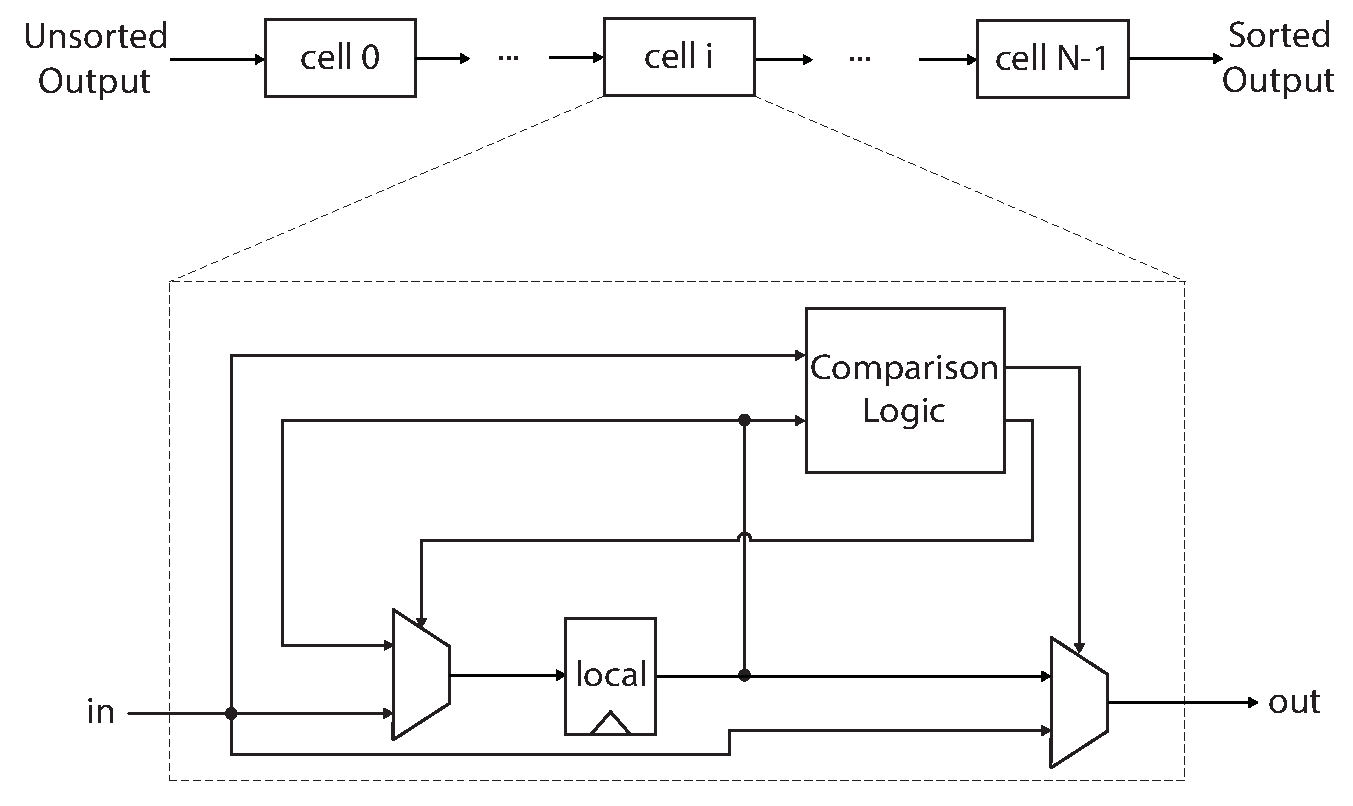
\includegraphics[width= \textwidth]{images/insertion_cell}
\caption{ The architecture of one insertion cell. Each cell holds exactly one value in the register \lstinline{local}. On each execution it receives an input value \lstinline{in}, compares that to its \lstinline{local} value, and writes the smaller of the two to \lstinline{output}. Sorting \lstinline{N} values requires \lstinline{N} cells. }
\label{fig:insertion_cell}
\end{figure}

Figure~\ref{fig:insertion_cell} shows a \gls{systolic_array} implementing insertion sort. Each cell is identical and compares its input (\lstinline{in}) with the value in current register \lstinline{local}. The smaller value is passed to the output \lstinline{out}, while the larger value is stored back in \lstinline{local}. In other words, \lstinline{out = min(in,local)}.  The output of cell $i$ is passed as input to the next cell $i+1$ in the linear array. As a new input arrives it will be compared against elements stored in the array until it finds it's correct place.  If a new input is larger than all of the  values in the array, then the sorted values will shift one cell to the right.  If a new input is smaller than all of the values in the array, then it will propagate through the array, and eventually become stored in the furthest right cell. After all the data has moved through the array, the smallest data element will be sorted in cell $N-1$ and can be read from the output. 

\begin{figure}
\lstinputlisting[firstline=3, lastline=15]{examples/insertion_cell_sort.cpp}
\caption{  The \VHLS C code corresponding to one insertion cell \lstinline{cell0}. The other cells have the exact same code except with a different function name (\lstinline{cell1}, \lstinline{cell2}, etc.). The code performs the same functionality as shown in the architectural diagram in Figure \ref{fig:insertion_cell}. It uses the \lstinline{hls:stream} interface for the input and output variables. \lstinline{hls::stream} provides a convenient method to create FIFOs that work both for synthesis and simulation. }
\label{fig:insertion_cell_sort.cpp}
\end{figure}

The code for one insertion cell is shown in Figure \ref{fig:insertion_cell_sort.cpp}. The code uses a streaming interface by declaring the input and output variables as an \lstinline{hls::stream} type. \lstinline{DTYPE} is a type parameter enabling different types to be operated on. The \lstinline{local} variable stores one element of the array being sorted. It is \lstinline{static} because we want to preserve its value across multiple function calls. This does create a problem since we must replicate this \lstinline{cell} function \lstinline{N} times.  Using the same function (e.g., calling the same \lstinline{cell} function N times) would cause a problem since each cell must have a separate static variable.  One static variable cannot be shared across N functions.

%\begin{figure}
%\lstinputlisting{examples/insertion_cell_sort.cpp}
%\caption{  The \VHLS C++ code defining an objecct representing one insertion cell \lstinline{cell0}.   }
%\label{fig:insertion_cell_object.cpp}

%\end{figure}
%A good solution to this problem is to use a C++ class to represent the systolic cell.  This code is shown in Figure \ref{fig:insertion_cell_object.cpp}

Linking the insertion cells together is straightforward. The function \lstinline{insertion_cell_sort} in Figure \ref{fig:partial_insertion_cell_sort.cpp} shows the code for sorting eight elements. Expanding this to a larger number of elements simply requires replicating more \lstinline{cell} functions, additional \lstinline{hls::stream} variables, instantiating these functions, and connecting their input and output function arguments in the appropriate manner.

\begin{figure}
\lstinputlisting{examples/partial_insertion_cell_sort.cpp}
\caption{  Insertion cell sorting for eight elements. The function takes an input \lstinline{hls::stream} and outputs the elements in sorted order one at a time through the variable \lstinline{out}. The order starts with the smallest element first, and then continues on to increasingly larger elements. }
\label{fig:partial_insertion_cell_sort.cpp}
\end{figure}

\begin{exercise}
The existing implementation of \lstinline{insertion_cell_sort} outputs the data starting with the smallest element and continues outputting increasingly larger elements. What changes are required in order to reverse this order, i.e., to output the largest element first, and then the decreasingly smaller outputs? 
\end{exercise}

The \lstinline{insertion_cell_sort} function must be called multiple times in order to sort the entire data. Each call to \lstinline{insertion_cell_sort} provides one data element to the array for sorting. The first call places the input data in its appropriate place. Where would this data be placed? To answer that question, we should point out that we make an assumption on the input data since we are initializing the \lstinline{local} variable to \lstinline{0}. This is done in all of the \lstinline{cell} functions.

\begin{exercise}
Initializing the \lstinline{static} variable \lstinline{local} to \lstinline{0} makes an assumption on the type of data that will be provided for sorting. What is this assumption? In other words, what is the range of values for the input data that will be properly handled? What would happen if input data from outside of this range was given to the \lstinline{insertion_cell_sort} function? Is there a better way to initialize the \lstinline{local} variable?
\end{exercise}

After making eight calls to the \lstinline{insertion_cell_sort} function, all of the data will be put into the eight \lstinline{local} variables in each of the \lstinline{cell} functions. 

\begin{exercise}
How many times must we call the \lstinline{insertion_cell_sort} function in order to get the first sorted element? How many calls are necessary in order to all of the sorted data? What if we increased the array to \lstinline{N} cells? Can you generalize these two functions (number of times to call \lstinline{insertion_cell_sort} to load \lstinline{N} elements, and the number of calls required to output all \lstinline{N} elements)?
\end{exercise}

To achieve a task-pipelined architecture consisting of the eight \lstinline{cell} functions, the code specifies the \lstinline{dataflow} directive. Each execution of the toplevel function processes a new input sample and inserts it into the sorted sequence.  The actual insertion is pipelined, with one pipeline stage for each call to the \lstinline{cell} function. With eight calls to the \lstinline{cell} function, we can only sort sequences with eight values, but this can be extended almost arbitrarily since the code contains no recurrences between the cells.

\begin{exercise}
How many cycles are required to sort an entire array? We define the sorting to be completed when all of the sorted data is output from the array of \lstinline{cell} function inside of the \lstinline{insertion_cell_sort}, i.e., all eight elements have been output from argument \lstinline{out} in the function \lstinline{insertion_cell_sort}? How does the cycle count change if we remove the \lstinline{dataflow} directive? How does change the resource utilization?
\end{exercise}

Figure \ref{fig:insertion_cell_sort_test.cpp} shows the code for the testbench. The testbench generates random data to be sorted in \lstinline{input[]}. This array is sorted by calling the \lstinline{insertion_cell_sort()} function multiple times, with the result appearing in \lstinline{cell_output[]}. Next, the same data is sorted in place using the \lstinline{insertion_sort} function from Figure \ref{fig:insertion_sort.cpp}. Finally, the testbench compares the results of these two sort implementations. The testbench passes if the sorted order from both implementations is the same.

\begin{figure}
\footnotesize\lstinputlisting[format=none]{examples/insertion_cell_sort-top.cpp}
%\end{figure}
%\begin{figure}
%\lstinputlisting[format=none,firstline=70]{examples/insertion_cell_sort-top.cpp}
\caption{  The testbench for the \lstinline{insertion_cell_sort} function. }
\label{fig:insertion_cell_sort_test.cpp}
\end{figure}

In the testbench, the \lstinline{SIZE} constant is set to the number of elements being sorted. This would be \lstinline{8} in the running example throughout this chapter. The \lstinline{DEBUG} constant is used to provided output detailing the execution of the testbench. This should be set to a non-zero value if you wish to see the debugging data, and \lstinline{0} if you want the output to be quiet. The input data is randomly generated using the \lstinline{rand()} function and stored in the \lstinline{input[]} array. You can change the data by modifying the argument in the call to \lstinline{srand()}.  The argument sets the seed for the random number generator to a specific value to ensure the generation of the same sequence of random numbers on each execution.  Changing this value to a different integer will result in a different, but predictable, random sequence.

Note again that the testbench calls the \lstinline{insertion_cell_sort()} function a total of \lstinline{SIZE*2} times. Each of the first \lstinline{SIZE} function calls feeds a single input element into function, but produce no useful output. The next \lstinline{SIZE} calls provide dummy input data and produce one sorted element each function call.  The data is produced one at a time starting with the smallest element.

\begin{exercise}
After executing a sort, the code in Figure \ref{fig:insertion_cell_sort.cpp} leaves the \lstinline{local} variable in a different state than when it started.  Unfortunately, this means that we can only sort one array! In most cases, we not only want to sort more than one array, but we'd like to process each array back to back with no bubbles in the pipeline.   Modify the code and the testbench to enable this and demonstrate that your modified code can sort multiple arrays.
\end{exercise}

\section{Merge Sort}
\label{sec:sort:merge}
Merge sort is a stable, divide and conquer algorithm invented by John von Neumann in 1945 \cite{knuth1998art}. The basic idea of the merge sort algorithm is that combining two sorted arrays into a larger sorted array is a relatively simple operation, which can be completed in $\mathcal{O}(n)$ time.    Conceptually, we divide the array into two subarrays, sort each subarray, and then combine the sorted subarrays into the final result. 

\begin{figure}
\centering
\setlength{\fboxsep}{1pt}
\begin{tabular} {l l l } 
width = 1, A[] = \{\colorbox{black!10}{3},\colorbox{black!10}{7},\colorbox{black!10}{6},\colorbox{black!10}{4},\colorbox{black!10}{5},\colorbox{black!10}{8},\colorbox{black!10}{2},\colorbox{black!10}{1}\} \\
width = 2, A[] = \{\colorbox{black!10}{3,\hspace*{2\fboxsep}7},\colorbox{black!10}{4,\hspace*{2\fboxsep}6},\colorbox{black!10}{5,\hspace*{2\fboxsep}8},\colorbox{black!10}{1,\hspace*{2\fboxsep}2}\} \\
width = 4, A[] = \{\colorbox{black!10}{3,\hspace*{2\fboxsep}4,\hspace*{2\fboxsep}7,\hspace*{2\fboxsep}6},\colorbox{black!10}{1,\hspace*{2\fboxsep}2,\hspace*{2\fboxsep}5,\hspace*{2\fboxsep}8}\} \\
width = 8, A[] = \{\colorbox{black!10}{1,\hspace*{2\fboxsep}2,\hspace*{2\fboxsep}3,\hspace*{2\fboxsep}4,\hspace*{2\fboxsep}5,\hspace*{2\fboxsep}6,\hspace*{2\fboxsep}7,\hspace*{2\fboxsep}8}\} \\
\\
\end{tabular}
\caption{The Merge Sort algorithm operating on an array.  The initial state where each element is considered to be a sorted subarray of length one is shown at the top.   At each step of the algorithm, subarrays are merged placing the shaded elements are in sorted order.}
\label{fig:merge_sort_behavior}
\end{figure}

Since we focus on sorting arrays of data, it turns out that the `divide' operation is actually trivial.  It requires no arithmetic or data movement and we can simply consider each individual element of the input array as a trivially sorted subarray.  All of the computation is involved with merging subarrays into larger sorted subarrays.  With other data representations, such as a linked-list, dividing an input array into subarrays can require traversing the data structure.   The merge sort process is shown in Figure \ref{fig:merge_sort_behavior}.  

\begin{figure}
\centering
\setlength{\fboxsep}{0pt}
\begin{tabular} {l l l } 
in1[] = \{\underline{3}, 4, 6, 7\} & in2[] = \{\underline{1}, 2, 5, 8\} & out[] = \{ \} \\
in1[] = \{\underline{3}, 4, 6, 7\} & in2[] = \{\colorbox{black}{1}, \underline{2}, 5, 8\}  & out[] = \{1\} \\
in1[] = \{\underline{3}, 4, 6, 7\} & in2[] = \{\colorbox{black}{1}, \colorbox{black}{2}, \underline{5}, 8\} & out[] = \{1, 2\} \\
in1[] = \{\colorbox{black}{3}, \underline{4}, 6, 7\} & in2[] = \{\colorbox{black}{1}, \colorbox{black}{2}, \underline{5}, 8\} & out[] = \{1, 2, 3\} \\
in1[] = \{\colorbox{black}{3}, \colorbox{black}{4}, \underline{6}, 7\} & in2[] = \{\colorbox{black}{1}, \colorbox{black}{2}, \underline{5}, 8\}  & out[] = \{1, 2, 3, 4\} \\
in1[] = \{\colorbox{black}{3}, \colorbox{black}{4}, \underline{6}, 7\} & in2[] = \{\colorbox{black}{1}, \colorbox{black}{2}, \colorbox{black}{5}, \underline{8}\}  & out[] = \{1, 2, 3, 4, 5\} \\
in1[] = \{\colorbox{black}{3}, \colorbox{black}{4}, \colorbox{black}{6}, \underline{7}\}  & in2[] = \{\colorbox{black}{1}, \colorbox{black}{2}, \colorbox{black}{5}, \underline{8}\}  &out[] = \{1, 2, 3, 4, 5, 6\} \\
in1[] = \{\colorbox{black}{3}, \colorbox{black}{4}, \colorbox{black}{6}, \colorbox{black}{7}\}  & in2[] = \{\colorbox{black}{1}, \colorbox{black}{2}, \colorbox{black}{5}, \underline{8}\}  &out[] = \{1, 2, 3, 4, 5, 6, 7\} \\
in1[] = \{\colorbox{black}{3}, \colorbox{black}{4}, \colorbox{black}{6}, \colorbox{black}{7}\}  & in2[] = \{\colorbox{black}{1}, \colorbox{black}{2}, \colorbox{black}{5}, \colorbox{black}{8}\} &out[] = \{1, 2, 3, 4, 5, 6, 7, 8\} \\
\end{tabular}
\caption{The process of merging two sorted arrays.  The initial state is shown at the top.  In each step of the algorithm, the underlined elements are considered and one is placed into sorted order in the output array.}
\label{fig:merge_behavior}
\end{figure}

The process of combining two sorted arrays into one larger sorted array is sometimes called the ``two finger algorithm''.  Figure \ref{fig:merge_behavior} describes the process using two sorted input arrays, named \lstinline{in1[]} and \lstinline{in2[]}. These are merged into a sorted output array, named \lstinline{out[]}.

The process starts with a ``finger'' pointing to the first element of each array.  This conceptual finger is just an index into the array storing the data.  As the algorithm proceeds, the fingers will point to different elements of the arrays. We underline these elements in order to show where the fingers are placed.  To begin with, the fingers point to the first element of each array, elements \lstinline{3} and \lstinline{1} in arrays \lstinline{in1[]} and \lstinline{in2[]}, respectively.

The first line of Figure \ref{fig:merge_behavior} shows the initial state. There are four elements in each of the two input arrays and zero elements in the output array. We compare the first two elements of the input arrays, and move the smaller of these two to the output array. In this case, we compare \lstinline{3} and \lstinline{1}, and move \lstinline{1} into \lstinline{out[]}. This reduces the number of elements in \lstinline{in2[]}, and our ``finger'' moves to the next element in \lstinline{in2[]} which is the next smallest element since the array is sorted. Once again, we compare the two elements from each of the input arrays, and move the smaller of the two elements to \lstinline{out[]}. In this case, we compare \lstinline{3} and \lstinline{2}, and move the element from \lstinline{in2[]} to \lstinline{out[]}. This process continues until all of the elements in one of the arrays is empty. In that case, we copy the remaining elements from the non-empty array into the output array.

Although the merge sort algorithm is a common textbook example of recursive function calls, most high-level synthesis tools do not support recursion or only support it in a limited manner. Thus, we will focus on a non-recursive implementation of the algorithm.  The code might look substantially different from what you are used to, but the core of the algorithm is exactly the same.

\subsection{Basic Merge Sort}

Figure \ref{fig:merge_sort.cpp} shows basic code implementing a non-recursive merge sort.  This code sorts an array by performing roughly $N \log N$ comparisons, but requires a temporary array to store the partially sorted data. The code starts by considering each element of the array as a length one sorted subarray.  Each iteration of the outer loop merges pairs of sorted subarrays into larger sorted subarrays.  After the first iteration we have sorted subarrays with maximum size 2, after the second iteration the sorted subarrays have maximum size 4, then 8 and so on.  Note that if the size of the input array is not a power of two, then it is possible that we might end up with some subarrays which are smaller than the maximum size.

\begin{figure}
\lstinputlisting{examples/merge_sort.cpp}
\caption{  A non-recursive implementation of merge sort. The \lstinline{merge_sort()} function iteratively merges subarrays until the entire array has been sorted. }
\label{fig:merge_sort.cpp}
\end{figure}

The sorting process starts in the \lstinline{merge_sort()} function. The function primarily operates on the input \lstinline{A[]} array, but leverages internal storage in \lstinline{temp[]}. The size of both of these arrays is determined by the \lstinline{SIZE} parameter. The parameter \lstinline{DTYPE} determines the type of data being sorted.

The computation of the function consists of two nested \lstinline{for} loops. The outer \lstinline{stage} loop keeps track of the number of elements in each sorted subarray in the \lstinline{width} variable. The function starts by considering each element as a separate subarray; hence \lstinline{width} is initialized as \lstinline{1}. Every iteration of the \lstinline{stage} loop results in the generation of longer sorted subarrays. These new subarrays potentially have twice as many elements, which is why \lstinline{width} doubles on each iteration of the \lstinline{stage} loop. The \lstinline{stage} loop terminates when \lstinline{width} is greater than or equal to \lstinline{SIZE}, indicating that all elements of \lstinline{A[]} are in a single sorted subarray.

Each iteration of the inner \lstinline{for} loop, labeled \lstinline{merge_arrays} merges two consecutive subarrays. These subarrays each consist of up to \lstinline{width} elements, starting at index \lstinline{i1} and \lstinline{i2}.  These two subarrays are merged and copied into a single subarray stored in \lstinline{temp[]} using the \lstinline{merge()} function.  The main complexity here is dealing with the boundary condition at the end of the loop if \lstinline{SIZE} is not exactly a power of two.  In this case the subarrays might contain less than \lstinline{width} elements. After merging subarrays into \lstinline{temp[]}, the final loop copies the data back into \lstinline{A[]} for the next iteration of the loop.

\begin{exercise}
The code in Figure \ref{fig:merge_sort.cpp} attempts to handle a wide variety of values for the parameter \lstinline{SIZE}.  What values are allowed?  When the \lstinline{merge()} function is called, whare are the possible relationships between \lstinline{i1}, \lstinline{i2}, and \lstinline{i3}?   If we restrict the allowed values of the parameter \lstinline{SIZE} can the code be simplified?  What is the affect on the resulting HLS generated circuit? 
\end{exercise}

The \lstinline{merge()} function performs the ``two finger'' algorithm on two subarrays within the \lstinline{in[]} array.  The function takes input in the \lstinline{in[]} array and produces output in the \lstinline{out[]} array. The function also takes as input variables \lstinline{i1}, \lstinline{i2}, and \lstinline{i3} which describe the extent of the two subarrays to be merged.  One subarray starts at index \lstinline{i1} and includes all the elements before \lstinline{i2} and the second subarray starts at index \lstinline{i2} and includes the elements up to \lstinline{i3}.  The merged output subarray will be stored from index \lstinline{i1} up to \lstinline{i3} in \lstinline{out[]}. 

The \lstinline{merge()} function consists of a single loop which iterates over the elements being stored into \lstinline{out[]}.  Each iteration places an element into its correctly sorted location in \lstinline{out[]}. The variables \lstinline{f1} and \lstinline{f2} within the function correspond to the position of the fingers for each subarray.  The \lstinline{if} condition selects the smaller of \lstinline{in[f1]} or \lstinline{in[f2]} to copy to the next sorted position in 
\lstinline{out[]}.  However, the \lstinline{if} condition is more complex since it has to deal with several special cases.  One case is where \lstinline{f1 == i2} and we have run out of elements to consider for \lstinline{in[f1]}, in which case we must select \lstinline{in[f2]} as the smallest element.  Alternatively, if \lstinline{f2 == i3}, then we  have run out of elements to consider for \lstinline{in[f2]}, in which case we must select \lstinline{in[f1]} as the smallest element.

\begin{exercise}
What happens to the \lstinline{in[]} array over the course of the computation? Describe the state of the elements in the \lstinline{in[]} array after each iteration of the outer \lstinline{for} loop. What is the final order of the elements in the \lstinline{in[]} array when \lstinline{merge_sort()} returns?
\end{exercise}

\begin{exercise}
The performance report after synthesis may not be able to determine the number of cycles for the latency and interval. Why is that the case? What are appropriate  \lstinline{min}, \lstinline{max}, and \lstinline{avg} values to provide in a \lstinline{loop_tripcount} directive(s)?
\end{exercise}

The code is not particularly optimized for any particular \gls{hls} implementation. The best starting point for optimization is by adding directives. Given that we have several nested \lstinline{for} loops, we generally look first at optimizing the inner loops.  Optimizations of inner loops are usually much more significant than optimizations of outer loops, which are executed relatively rarely. By this point, you should be familiar with the common \lstinline{pipeline} and \lstinline{unroll} directives for loop optimization. 

\begin{exercise}
Perform different optimizations using the \lstinline{pipeline} and \lstinline{unroll} directives on the \lstinline{for} loops. What provides the best performance? Which gives the best tradeoff between resource utilization and performance?  What aspects of the code prevent higher performance?  Are these aspects fundamental to the algorithm, or only because of the way the algorithm is captured in the code?
\end{exercise}

Pipelining and unrolling can be hindered by resource constraints; in particular, we must carefully consider the number of memory ports for the arrays. The arrays in this code seem relatively straightforward as they are both one-dimensional. Yet, the designer must carefully consider the access patterns to insure that performance optimizations match with the resource constraints. 

\begin{exercise}
Optimize the code using loop optimizations and array partitioning, i.e., create a set of designs using the \lstinline{array_partition}, \lstinline{pipeline}, and \lstinline{unroll} directives. Were you able to achieve better results than by using the \lstinline{pipeline} and \lstinline{unroll} directives alone? What was the best strategy for performing design space exploration using these directives? What was your best design in terms of performance? What was the best design that provides a good tradeoff between resource utilization and performance?
\end{exercise}

Many times the best designs are only possible by performing code restructuring. Although \VHLS provides many directives to enable common code optimizations, it is impractical to provide directives for every optimization.  Sometimes we must resort to rewriting the code in addition to providing directives in order to achieve a design that meets our requirements.  In the next section we describe one way to significantly restructure the merge sort code in order to increase throughput.

\subsection{Restructured Merge Sort}
Looking first at the inner loop of the \lstinline{merge()} function, you might have found that it was difficult to achieve a loop II of 1.  One challenge is that there are actually four reads of \lstinline{in[]}, but only at two different addresses.   The HLS tool must recognize that these reads are redundant, since \gls{bram} memories can only support two accesses each clock.  However because these reads are in different basic blocks, it is more difficult for a compiler to eliminate the redundant loads.  By eliminating the redundant reads, the compiler needs to do less optimization to achieve a loop II of 1.  The restructured code is shown in Figure \ref{fig:merge_sort_restructured.cpp}.  In addition, there is a recurrence through the \lstinline{f1} and \lstinline{f2} variables.  These variables are incremented in one of the branches of the \lstinline{if} conditional, which must be used in the next iteration to determine which locations in \lstinline{in[]} to compare and subsequently which branch of the conditional to take.  Because the floating point comparison is relatively complex, this recurrence can also limit the achievable II and clock period.

\begin{figure}
\lstinputlisting[format=none, lastline=23]{examples/merge_sort_restructured.cpp}
\caption{Restructured code for the \lstinline{merge()} function, which can achieve a loop II of 1 in \VHLS.}
\label{fig:merge_sort_restructured.cpp}
\end{figure}

The behavior of this code is shown in Figure \ref{fig:merge_sort_restructured_behavior}.  Although the inner loop achieves a loop II of 1, this inner loop often has a very small number of loop iterations.  When the inner loop finishes, the pipeline must empty before code executing after the pipeline can execute.  Although the loop pipeline is relatively short in this case, the bubble caused by the loop completing is significant, since the number of iterations is also small.  Unfortunately, because of the limits of static loop analysis, the performance of this particular code is somewhat hard to visualize.  In this case, the number of iterations of the inner loop is data dependent.

\begin{figure}
\centering
\includesvg{merge_sort_restructured_behavior}
\caption{Behavior of the restructured code in Figure \ref{fig:merge_sort_restructured.cpp}.}
\label{fig:merge_sort_restructured_behavior}
\end{figure}

A common approach is to flatten loop nests like these into a single loop, reducing the number of times that the pipeline must flush when exiting a loop.  In fact, \VHLS will automatically flatten perfect loop nests.  In this case, however, since the code does not contain a perfect loop nest, we can resort to flattening the loops manually.  Code resulting from manually flattening the \lstinline{merge_arrays} loop with the loop inside the \lstinline{merge()} function is shown in Figure \ref{fig:merge_sort_loop_merged.cpp}.  Note that one advantage of this code is that the \lstinline{merge_arrays} loop also has a constant number of loop iterations, making understanding performance much easier.

\begin{figure}
\lstinputlisting[format=none]{examples/merge_sort_loop_merged.cpp}
\caption{Restructured code for Merge Sort which can achieve a loop II of 1 with fewer pipeline bubbles in \VHLS.}
\label{fig:merge_sort_loop_merged.cpp}
\end{figure}

\begin{aside}
Estimate the performance of the code in Figure \ref{fig:merge_sort_loop_merged.cpp}.  Even though the inner loops have achieved a loop II of 1, is the design using hardware efficiently?  Is there a way to further reduce the latency of the \lstinline{merge_sort()} function to the point where it is using approximately $N \log N$ clock cycles?
\end{aside}

So far we have focused on optimizing the \lstinline{merge_sort()} function to reduce the latency of the computation without significantly increasing the number of resources.   As a result, the accelerator is becoming more efficient.  However, after achieving a reasonably efficient design, the only way to further reduce latency and/or increase throughput is increase parallelism.  Previously we have seen ways of unrolling inner loops and partitioning arrays as a way to perform more work each clock cycle.  An alternative way to increase parallelism is leverage pipelining.  In addition to operator-level pipelinling we can also look for coarser-granularity task-level pipelining.

With Merge Sort it turns out that we can make a dataflow pipeline out of each iteration of the \lstinline{stage} loop, assuming that we have a fixed size array to sort.  In \VHLS this implementation can be conceptually achieved by unrolling the \lstinline{stage} loop and using the \lstinline{dataflow} directive.  Each instance of the \lstinline{merge_arrays} loop then becomes an independent process which can operate on a different set of data.  The resulting architecture is shown in Figure \ref{fig:restructured_mergesort_dataflow}.  

\begin{figure}
\centering
\includesvg{restructured_mergesort_dataflow}
\caption{Dataflow pipelined architecture for implementing 4 stages of Merge Sort.  This architecture can sort up to 16 elements.}
\label{fig:restructured_mergesort_dataflow}
\end{figure}

\begin{figure}
\footnotesize
\lstinputlisting{examples/merge_sort_parallel.cpp}
\caption{Restructured code for Merge Sort which can be implemented as a dataflow pipeline by \VHLS.}
\label{fig:merge_sort_parallel.cpp}
\end{figure}

The code to implement this is shown in Figure \ref{fig:merge_sort_parallel.cpp}.  This code is similar in many ways to the original code, but has several important differences.  One key difference is that the \lstinline{merge_arrays} loop has been extracted into a function, making it easier simpler to rewrite the toplevel code. A second key difference is that the output of \lstinline{merge_sort_parallel()} is produced in a separate array than the input, enabling \VHLS to build an architecture that pipelined architecture processing using the \lstinline{dataflow} directive.  Additionally, the \lstinline{temp[][]} array is now used to model the dataflow ping-pong channels between the processes implemented by the \lstinline{merge_arrays()} function, making extra array copies unnecessary.  This two-dimensional array is partitioned in the first dimension, making it easy to represent a parameterized number of channels.

The \lstinline{merge_sort_parallel()} function consists of \lstinline{STAGES} calls to the \lstinline{merge_arrays()} function.  Each The first call reads from the input and writes to \lstinline{temp[0]}.  The loop performs the intermediate stages  and writes to the remaining partitions of \lstinline{temp[]}.  The final call writes to the output array \lstinline{B[]}.  The code is parameterized in terms of \lstinline{SIZE} and \lstinline{STAGES} and supports array lengths 4 or greater.

\begin{aside}
Estimate the performance of the code in Figure \ref{fig:merge_sort_parallel.cpp}.  What is the interval and latency of the implementation?  How much memory is required to support that processing rate?   Is all of the memory necessary?
\end{aside}

\section{Conclusion}

This chapter introduced a number of basic sorting algorithms with fundamentally different algorithmic tradeoffs.  Insertion sort operating on an array performs on average $N^2/4$ comparisons, but requires much fewer (approximately $N$ comparisons) when operating on sorted data. We showed several ways of parallelizing Insertion sort which can increase performance at the expense of using more hardware resources.  Because of bubbles in the statically scheduled pipeline, we end up needing roughly $N$ comparators with an interval of $N$ cycles to perform insertion sort.  Merge sort operating on an array performs generally fewer comparisons, roughly $N \log N$, but requires additional memory to store partially sorted results.  The more complex loop structure of Merge Sort means that we required additional refactoring to reach an efficient solution that took roughly $N \log N$ cycles with one comparator.  We also showed a task-pipelined implementation which performs $\log N$ comparisons every clock cycle with an interval of $N$ cycles to perform merge sort.  In contrast with insertion sort, this requires much fewer comparisons to achieve the same interval, but requires more memory (in the form of dataflow channels) and has much higher latency.

In practice, many FPGA-based implementations of sorting will have to address these fundamental tradeoffs in order to achieve the best integration with other aspects of a system. Another sort with a fundamentally different tradeoff is the Radix Sort, which focuses on data that exists within a bounded range, unlike the more general sorting algorithms in this chapter which only require comparison between items.  Radix sort will be implemented as part of the Huffman Coding in Chapter \ref{chapter:huffman}.

Parallel implementations of sorting algorithms are often described as sorting networks.  Sorting networks are sometimes described as \glspl{systolic_array} and other times as pipelines.  We can often gain inspiration for HLS designs by looking investigating these existing parallel implementations and then capturing them as C code.  In \VHLS, these networks can be described using either loop pipelines, dataflow pipelines, or a combination of both.
 
%\note{From Janarbek: Please look at : Templates \textbackslash sorting \textbackslash RadixSort \textbackslash RO2. And this one: MergeSort\textbackslash MergeCascadeStreaming \textbackslash 256. I  expect these two algorithms to be at least small sub section or a section meaning that you can write a lot. These are especially merge sort is optimized.}
